% !TEX encoding = UTF-8
% !TEX TS-program = pdflatex
% !TEX root = ../tesi.tex

%**************************************************************
\chapter{Il contesto aziendale}
\label{cap:processi-metodologie}
%**************************************************************

%**************************************************************
\section{L'azienda: \textbf{\azienda}}
\azienda\ nasce nel 2013 come azienda focalizzata nello sviluppo di soluzioni basate sul comportamento in materia di sicurezza e anti frode. Nel 2014 ha rilasciato le prime soluzioni sulla protezione ed analisi delle transazioni finanziarie.\\
XTN è situata in tre diverse sedi nel nord Italia, Padova, Milano e Rovereto. Attualmente è attiva  nello sviluppo di soluzioni \emph{B2B}\glsfirstoccur sia in ambito anti frode che di applicazioni per la protezione di dispositivi mobile e IoT.\\
  
\section{Prodotti offerti}
\azienda\ offre 2 prodotti di punta, \textbf{Smash\textregistered} e \textbf{More\textregistered}.\\
\\
\textbf{Smash\textregistered} è un \emph{framework}\glsfirstoccur\ che analizza il comportamento abituale, grazie a più di cento parametri, degli utenti di servizi di pagamento online. Grazie a questa funzionalità riesce a stabilire, in tempo reale, il fattore di rischio di ogni transazione.\\
Il fattore di rischio è calcolato attraverso svariati algoritmi comportamentali personalizzabili dall'utente tramite un apposito \textit{editor} integrato alla piattaforma. Se, grazie a questi algoritmi, una transazione dovesse risultare sospetta, questa verrà notificata ad una persona incaricata a verificarne l'effettiva natura.\\
Non vengono analizzate solamente i parametri delle transazioni, ad esempio il destinatario o la geocalizzazione, ma anche fattori esterni come anomalie nei protocolli di comunicazione, manipolationi html, compromissioni del dispositivo mobile.\\
Questo prodotto è destinato a istituti finanziari, negozi online e assicurazioni.\\
\\
\textbf{More\textregistered} invece è un servizio installabile nei dispositivi mobili in grado di verificare se l'utente che sta utilizzando il dispositivo, in un determinato istante, coincide con l'utente che dice di essere. Questo è possibile analizzando molteplici parametri, tra cui lo stato del dispositivo, correlandoli poi con un analisi comportamentale e biometrica.\\
More\textregistered\ è installabile in una qualsiasi applicazione mobile che contine informazioni informazioni confidenziali o critiche, come ad esempio un'applicazione bancaria.\\
Tutte le operazioni necessarie per il funzionamento di More\textregistered\ sono eseguite in ambiente \textit{clound} preservanzo, quindi, le prestazioni dell'applicazione che lo ospita.
\newpage

\section{Organizzazione aziendale}
XTN adotta l'\textit{agile team organisation} tramite \textit{Squads, Chapters, Guilds}.
\begin{figure}[ht]
	\centering
	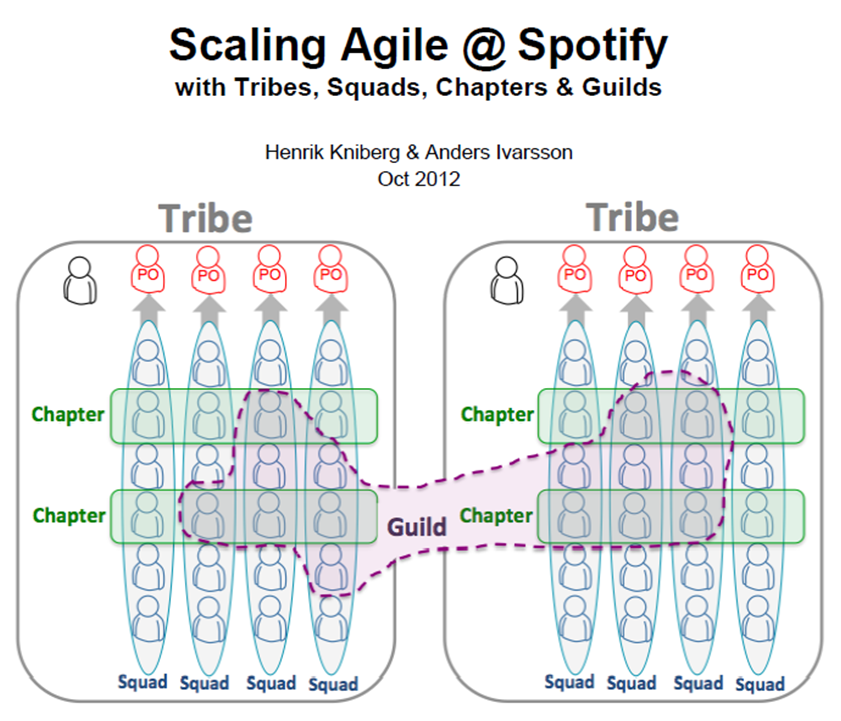
\includegraphics[scale=0.80]{immagini/agile-org.png}
	\caption{\textit{Agile team organisation}}
\end{figure}
\begin{itemize}
\item{\textbf{Squads}:} sono un gruppo di persone che condividono il luogo di lavoro ed il campo di interesse. In XTN esistono due squads rispettivamente uno per  Smash\textregistered\ ed uno per More\textregistered. Ogni squads ha il proprio \textit{project manager}, ed essi si riuniscono periodicamente, ogni settimana, per tracciare e discutere la situaione delle varie \textit{milestone}. 
\item{\textbf{Chapters}:} sono un gruppo di persoone che condividono le competenze, trasversalmente tra i vari squads, per promuovere l'innovazione e la collaborazione. Periodicamente, circa ogni mese, i vari chapters si riuniscono per convidivere informazioni di interesse e favorire un allineamento tecnologico tra i vari squads.
\item{\textbf{Guilds}:} sono una comunità di membri, in tutta l'organizzazione, che vogliono condividere conoscenze, strumenti e pratiche comuni. Ad esempio, in XTN, eiste una \textit{guild} nata per accrescere la conoscienza sull'intelligenza artificiale.
\item{\textbf{Tribe}:} sono nate per suddividere, e rendere piu gestibile, una grande infrastruttura. XTN non ha addottato questo concetto essendo ancora un azienda di piccole dimensioni.
\end{itemize}

\section{Processi aziendali}
In questa sezioni verranno affrontati i processi aziendali che ho avuto modo conoscere ed imparare lavorando a stretto contatto con il team di Smash\textregistered.
\subsection{Processo di sviluppo}
L'azienda si ritrova spesso a dover vendere il proprio prodotto con un certo numero di personalizzazioni. Per far ciò gli addetti alla vendita, di XTN, effettuano incontri con i clienti per ricavare idee ed osservazioni per, successivamente, stilarli in un documento. Questo documeto poi verrà usato dal team di sviluppo per creare il prodotto in linea con le richieste del cliente.\\
Non vengono rilasciati protipi incompleti al cliente ma solamente prodotti funzionanti con tutte le personalizzazioni richieste.\\
Attualmente ogni personalizzazione richiesta dal cliente, il team di sviluppo, cerca di renderele delle \textit{feauture} usabili da tutti e quindi rivendibili.\\
\subsection{Gestione della configurazione}
Tutte le configurazioni sono mantenute in un repository interno in modo da gestirne le varie parti e tener traccia delle modifiche. Prima di essere aggiunte al repository interno, le varie configurazioni, devono essere verificate dall'amministratore di progetto.
\subsection{Processo di manutenzione}
Ogni mulfunzionamento viene segnalato e tracciato con la rispettiva priorità. Il personale addetto risolverà le varie segnalazioni in ordine di priorità e successivamente, dopo avere sistemato un certo numero di malfunzionamenti, il \textit{project manager} rilascerà la nuova versione del prodotto.
\subsection{Processo di verifica}
Il processo viene gestito dal \textit{chapter} che garantisce la qualità del prodotto offerto.
\section{Strumenti a supporto dei processi}
In questa sezione verranno elencati le principali tecnologie, a supporto dei processi, utilizzate nel prodotto Smash\textregistered.
\subsection{Processo di sviluppo}
\subsubsection{Backend}
Per quanto riguarda la parte logica l'azienda ha deciso di utilizzare principalmente Java come linguaggio, in quanto è molto performante ed ha una sintassi molto regolare. Per quest'ultimo il team di sviluppo ha deciso di adottare il \textit{framework Spring} per astrarre, e semplificare, buona parte di architettura di \textit{backend}.\\
Per quanto riguarda la persistenza dei dati, XTN, ha deciso di adottare MongoDB.
\subsection{Processo di configurazione}
Per tener traccia di tutte le modifiche ed evitare sovrascritture involontarie l'azienda ha deciso di adottare una repository interna chiamata Stash. Quest'ultima è un sistema di gestione di repository che utilizzano diversi sistemi di controllo di versione, tra cui Git e Mercurial. Infine l'azienda ha deciso di utilizzare Git come controllo di versione.
\subsection{Processo di manutenzione}
Qualunque malfunzionamento viene segnalato e registrato in un sistema di tracciamento delle \textit{issues} chiamato Jira. Questo servizio permette di assegnare, per ogni \textit{issues}, una priorità, una scadenza e la versione con cui il malfunzionamento sarà sistemato. 
\section{Rapporto con l'innovazione}


